\documentclass{article}
\usepackage{tikz}

\begin{document}

\begin{figure}[h]
    \centering
    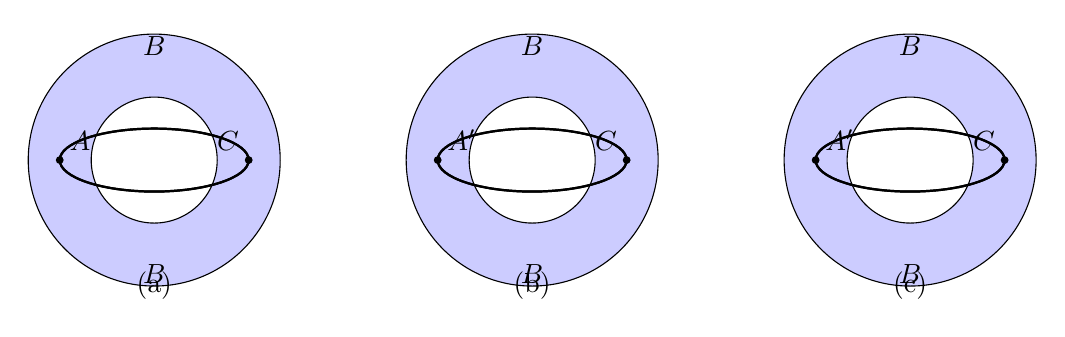
\begin{tikzpicture}[scale=0.8]
        % Diagram (a)
        \draw[fill=blue!20] (0,0) circle (2);
        \draw[fill=white] (0,0) circle (1);
        
        \draw[thick] (-1.5,0) arc (180:360:1.5 and 0.5);
        \draw[thick] (-1.5,0) arc (180:0:1.5 and 0.5);
        
        \draw[thick] (-1.5,0) arc (180:360:1.5 and 0.5);
        \draw[thick] (-1.5,0) arc (180:0:1.5 and 0.5);
        
        \node at (-1.5,0) [circle,fill,inner sep=1pt] {};
        \node at (1.5,0) [circle,fill,inner sep=1pt] {};
        
        \node at (-1.5,0) [above right] {$A$};
        \node at (1.5,0) [above left] {$C$};
        \node at (0,1.5) [above] {$B$};
        \node at (0,-1.5) [below] {$B$};
        
        \node at (0,-2) {(a)};
        
        % Diagram (b)
        \begin{scope}[xshift=6cm]
            \draw[fill=blue!20] (0,0) circle (2);
            \draw[fill=white] (0,0) circle (1);
            
            \draw[thick] (-1.5,0) arc (180:360:1.5 and 0.5);
            \draw[thick] (-1.5,0) arc (180:0:1.5 and 0.5);
            
            \draw[thick] (-1.5,0) arc (180:360:1.5 and 0.5);
            \draw[thick] (-1.5,0) arc (180:0:1.5 and 0.5);
            
            \node at (-1.5,0) [circle,fill,inner sep=1pt] {};
            \node at (1.5,0) [circle,fill,inner sep=1pt] {};
            
            \node at (-1.5,0) [above right] {$A'$};
            \node at (1.5,0) [above left] {$C$};
            \node at (0,1.5) [above] {$B$};
            \node at (0,-1.5) [below] {$B$};
            
            \node at (0,-2) {(b)};
        \end{scope}
        
        % Diagram (c)
        \begin{scope}[xshift=12cm]
            \draw[fill=blue!20] (0,0) circle (2);
            \draw[fill=white] (0,0) circle (1);
            
            \draw[thick] (-1.5,0) arc (180:360:1.5 and 0.5);
            \draw[thick] (-1.5,0) arc (180:0:1.5 and 0.5);
            
            \draw[thick] (-1.5,0) arc (180:360:1.5 and 0.5);
            \draw[thick] (-1.5,0) arc (180:0:1.5 and 0.5);
            
            \node at (-1.5,0) [circle,fill,inner sep=1pt] {};
            \node at (1.5,0) [circle,fill,inner sep=1pt] {};
            
            \node at (-1.5,0) [above right] {$A'$};
            \node at (1.5,0) [above left] {$C$};
            \node at (0,1.5) [above] {$B$};
            \node at (0,-1.5) [below] {$B$};
            
            \node at (0,-2) {(c)};
        \end{scope}
    \end{tikzpicture}
\end{figure}

\end{document}